                                                                               \documentclass[tikz]{standalone}
\usepackage{lmodern}
\usepackage[algoruled,vlined,linesnumbered,titlenotnumbered,noend]{algorithm2e}
\usepackage{color,amsmath,bm,bbm,stmaryrd,amssymb,pifont,bbding}
\usetikzlibrary{backgrounds}
\usetikzlibrary{calc} 

\usetikzlibrary{shapes}
\usetikzlibrary{shadows}
\usetikzlibrary{decorations.pathmorphing}
\usetikzlibrary{decorations.text}
\usetikzlibrary{decorations}
\usetikzlibrary{arrows,bending}
\usetikzlibrary{shapes.arrows}
\tikzset{nobg/.style={show background rectangle,background rectangle/.style={opacity=0}}}


\input ../../styles
\input ../../globalcomm
\usetikzlibrary{arrows, shapes.gates.logic.US, calc}

  \tikzstyle{bddnode}=[draw,rectangle,rounded corners=2mm]
  \tikzstyle{aops}=[pos=0.9,below,yshift=0mm,xshift=-2mm]
\begin{document}

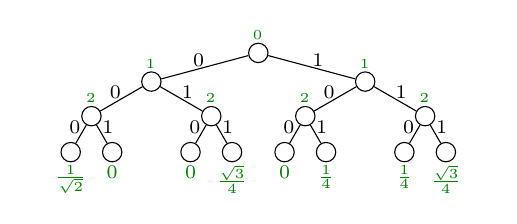
\begin{tikzpicture}
\node[circle,draw,name=ne,inner sep=0pt,minimum size=7pt] at (0,0){};
\node[anchor=south,font=\scriptsize,inner sep=1pt] at (ne.north) {\textcolor{green!50!black}{$\xvar_0$}};
%%%%%%%%%%%%%%%%%%%%%%%%%%%%%%%%%%%%%%%%%%%%%%%%%%%%%%%%%%%%%%%

\node[circle,draw,name=n0,inner sep=0pt,minimum size=7pt] at
($(ne)+(195:40pt)$){};
\node[anchor=south,inner sep=1pt,font=\scriptsize] at (n0.north) 
{\textcolor{green!50!black}{$\xvar_1$}};

\node[circle,draw,name=n00,inner sep=0pt,minimum size=7pt] at 
($(n0)+(210:25pt)$){};
\node[anchor=south,inner sep=1pt,font=\scriptsize] at (n00.north) 
{\textcolor{green!50!black}{$\xvar_2$}};



\node[circle,draw,name=n000,inner sep=0pt,minimum size=7pt] at ($(n00)+(240:15pt)$){};
\node[anchor=north,inner sep=1pt,font=\scriptsize] at (n000.south) 
{\textcolor{green!50!black}{$\frac{1}{\sqrt2}$}};



\node[circle,draw,name=n001,inner sep=0pt,minimum size=7pt] at ($(n00)+(300:15pt)$){};
\node[anchor=north,inner sep=1pt,font=\scriptsize] at (n001.south) 
{\textcolor{green!50!black}{$0$}};


\node[circle,draw,name=n01,inner sep=0pt,minimum size=7pt] at
($(n0)+(330:25pt)$){};
\node[anchor=south,inner sep=1pt,font=\scriptsize] at (n01.north) 
{\textcolor{green!50!black}{$\xvar_2$}};

\node[circle,draw,name=n010,inner sep=0pt,minimum size=7pt] at ($(n01)+(240:15pt)$){};
\node[anchor=north,inner sep=1pt,font=\scriptsize] at (n010.south) 
{\textcolor{green!50!black}{$0$}};

\node[circle,draw,name=n011,inner sep=0pt,minimum size=7pt] at ($(n01)+(300:15pt)$){};
\node[anchor=north,inner sep=1pt,font=\scriptsize] at (n011.south) 
{\textcolor{green!50!black}{$\frac{\sqrt3}{4}$}};

\node[circle,draw,name=n1,inner sep=0pt,minimum size=7pt] at
($(ne)+(345:40pt)$){};
\node[anchor=south,inner sep=1pt,font=\scriptsize] at (n1.north) 
{\textcolor{green!50!black}{$\xvar_1$}};
%%%%%%%%%%%%%%%%%%%%%%%%%%%%%%%%%%%%%%%%%%%%%%%%%%%%%%%%%%%%%%%

\node[circle,draw,name=n10,inner sep=0pt,minimum size=7pt] at 
($(n1)+(210:25pt)$){};
\node[anchor=south,inner sep=1pt,font=\scriptsize] at (n10.north) 
{\textcolor{green!50!black}{$\xvar_2$}};

\node[circle,draw,name=n100,inner sep=0pt,minimum size=7pt] at ($(n10)+(240:15pt)$){};
\node[anchor=north,inner sep=1pt,font=\scriptsize] at (n100.south) 
{\textcolor{green!50!black}{$0$}};

\node[circle,draw,name=n101,inner sep=0pt,minimum size=7pt] at ($(n10)+(300:15pt)$){};
\node[anchor=north,inner sep=1pt,font=\scriptsize] at (n101.south) 
{\textcolor{green!50!black}{$\frac{1}{4}$}};


\node[circle,draw,name=n11,inner sep=0pt,minimum size=7pt] at
($(n1)+(330:25pt)$){};
\node[anchor=south,inner sep=1pt,font=\scriptsize] at (n11.north) 
{\textcolor{green!50!black}{$\xvar_2$}};

\node[circle,draw,name=n110,inner sep=0pt,minimum size=7pt] at ($(n11)+(240:15pt)$){};
\node[anchor=north,inner sep=1pt,font=\scriptsize] at (n110.south) 
{\textcolor{green!50!black}{$\frac{1}{4}$}};

\node[circle,draw,name=n111,inner sep=0pt,minimum size=7pt] at ($(n11)+(300:15pt)$){};
\node[anchor=north,inner sep=1pt,font=\scriptsize] at (n111.south) 
{\textcolor{green!50!black}{$\frac{\sqrt3}{4}$}};


%%%%%%%%%%%%%%%%%%%%%%%%%%%%%%%%%%%%%%%%%%%%%%%%%%%%%%%%%%%%%%%


\draw[line width=0.4pt] (ne) -- 
node[anchor=south east,inner sep=0pt,font=\scriptsize]{$0$}
(n0);
\draw[line width=0.4pt] (ne)-- 
node[anchor=south west,inner sep=0pt,font=\scriptsize]{$1$}
(n1);

\draw[line width=0.4pt] (n0)-- 
node[anchor=south east,inner sep=0pt,font=\scriptsize]{$0$}(n00);
\draw[line width=0.4pt] (n00)--
node[anchor=south east,inner sep=0pt,font=\scriptsize]{$0$}(n000);
\draw[line width=0.4pt] (n00)--
node[anchor=south west,inner sep=0pt,font=\scriptsize]{$1$}
(n001);

\draw[line width=0.4pt] (n0)--
node[anchor=south west,inner sep=0pt,font=\scriptsize]{$1$}
(n01);
\draw[line width=0.4pt] (n01)-- 
node[anchor=south east,inner sep=0pt,font=\scriptsize]{$0$}
(n010);

\draw[line width=0.4pt] (n01)--
node[anchor=south west,inner sep=0pt,font=\scriptsize]{$1$}
(n011);

\draw[line width=0.4pt] (n1)-- 
node[anchor=south east,inner sep=0pt,font=\scriptsize]{$0$}
(n10);
\draw[line width=0.4pt] (n10)--
node[anchor=south east,inner sep=0pt,font=\scriptsize]{$0$}
(n100);
\draw[line width=0.4pt] (n10)--
node[anchor=south west,inner sep=0pt,font=\scriptsize]{$1$}
(n101);

\draw[line width=0.4pt] (n1)--
node[anchor=south west,inner sep=0pt,font=\scriptsize]{$1$}
(n11);
\draw[line width=0.4pt] (n11)--
node[anchor=south east,inner sep=0pt,font=\scriptsize]{$0$}
(n110);
\draw[line width=0.4pt] (n11)--
node[anchor=south west,inner sep=0pt,font=\scriptsize]{$1$}
(n111);


%%%%%%%%%%%%%%%%%%%%%%%%%%%%%%%%%%%%%%%%%%%%%%%%%%%%%%%%%%%%%%%

\node[name=leftmargin] at (-80pt,0pt){};
\node[name=rightmargin] at (80pt,0pt){};
\node[name=leftlevel1] at (leftmargin |- n0.west) {};
\node[name=rightlevel1] at (rightmargin |- n0.west) {};
%\draw[dotted] (leftlevel1) -- (rightlevel1);

\end{tikzpicture}


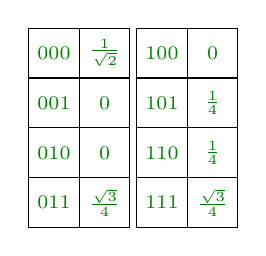
\begin{tikzpicture}
\node[line width=0.4pt,draw,name=n000,minimum width=7pt,minimum height=18pt,font=\scriptsize,anchor=north]
at (0,0)
{\textcolor{green!50!black}{$000$}};

\node[line width=0.4pt,draw,name=p000,minimum width=18pt,minimum height=18pt,font=\scriptsize,anchor=west]
at ($(n000.east)+(-0.4pt,0pt)$)
{\textcolor{green!50!black}{$\frac1{\sqrt2}$}};

\node[draw,name=n001,minimum width=7pt,minimum height=18pt,font=\scriptsize,anchor=north]
at ($(n000.south)+(0pt,0.4pt)$)
{\textcolor{green!50!black}{$001$}};

\node[line width=0.4pt,draw,name=p001,minimum width=18pt,minimum height=18pt,font=\scriptsize,anchor=west]
at ($(n001.east)+(-0.4pt,0pt)$)
{\textcolor{green!50!black}{$0$}};


\node[draw,name=n010,minimum width=7pt,minimum height=18pt,font=\scriptsize,anchor=north]
at ($(n001.south)+(0pt,0.4pt)$)
{\textcolor{green!50!black}{$010$}};

\node[line width=0.4pt,draw,name=p010,minimum width=18pt,minimum height=18pt,font=\scriptsize,anchor=west]
at ($(n010.east)+(-0.4pt,0pt)$)
{\textcolor{green!50!black}{$0$}};


\node[draw,name=n011,minimum width=7pt,minimum height=18pt,font=\scriptsize,anchor=north]
at ($(n010.south)+(0pt,0.4pt)$)
{\textcolor{green!50!black}{$011$}};

\node[line width=0.4pt,draw,name=p011,minimum width=18pt,minimum height=18pt,font=\scriptsize,anchor=west]
at ($(n011.east)+(-0.4pt,0pt)$)
{\textcolor{green!50!black}{$\frac{\sqrt 3}4$}};



\node[line width=0.4pt,draw,name=n100,minimum width=7pt,minimum height=18pt,font=\scriptsize,anchor=west]
at ($(n000.east)+(20pt,0pt)$)
{\textcolor{green!50!black}{$100$}};
\node[line width=0.4pt,draw,name=p1001,minimum width=18pt,minimum height=18pt,font=\scriptsize,anchor=west]
at ($(n100.east)+(-0.4pt,0pt)$)
{\textcolor{green!50!black}{$0$}};



\node[draw,name=n101,minimum width=7pt,minimum height=18pt,font=\scriptsize,anchor=north]
at ($(n100.south)+(0pt,0.4pt)$)
{\textcolor{green!50!black}{$101$}};
\node[line width=0.4pt,draw,name=p1001,minimum width=18pt,minimum height=18pt,font=\scriptsize,anchor=west]
at ($(n101.east)+(-0.4pt,0pt)$)
{\textcolor{green!50!black}{$\frac1 4$}};


\node[draw,name=n110,minimum width=7pt,minimum height=18pt,font=\scriptsize,anchor=north]
at ($(n101.south)+(0pt,0.4pt)$)
{\textcolor{green!50!black}{$110$}};
\node[line width=0.4pt,draw,name=p1001,minimum width=18pt,minimum height=18pt,font=\scriptsize,anchor=west]
at ($(n110.east)+(-0.4pt,0pt)$)
{\textcolor{green!50!black}{$\frac1 4$}};


\node[draw,name=n111,minimum width=7pt,minimum height=18pt,font=\scriptsize,anchor=north]
at ($(n110.south)+(0pt,0.4pt)$)
{\textcolor{green!50!black}{$111$}};
\node[line width=0.4pt,draw,name=p1001,minimum width=18pt,minimum height=18pt,font=\scriptsize,anchor=west]
at ($(n111.east)+(-0.4pt,0pt)$)
{\textcolor{green!50!black}{$\frac{\sqrt3} 4$}};

%%%%%%%%%%%%%%%%%%%%%%%%%%%%%%%%%%%%%%%%%%%%%%%%%%%%%%%%%%%%%%%

\end{tikzpicture}



\tikzstyle{mops}=[pos=0.9,above,yshift=1mm,xshift=-2mm]
\tikzstyle{bddnode}=[draw,rectangle,rounded corners=2mm]
\tikzstyle{bddnodex}=[bddnode,inner sep=1mm]
  \tikzstyle{hshift}=[xshift=7mm]
\tikzstyle{translow}=[->,>=stealth',dashed]
  \tikzstyle{trans}=[->,>=stealth']
  \tikzstyle{blueark}=[fill=blue,opacity=0.2]


\begin{tikzpicture}[node distance=20mm]

  %%%%%%%%%%%%%%% transition %%%%%%%%%%%%%%%%%%%
   \node[bddnodex] (p) {$p$};
  \draw (p) coordinate[yshift=-0mm,xshift=7mm] (pa);
  \node[bddnodex,below right of=p,hshift,yshift= 5mm] (q1+) {$q^1_+$};
  \node[bddnodex,above right of=p,hshift,yshift=-5mm] (q1+-) {$q^1_\pm$};
    
 \draw[translow] (pa)
    to[bend right=10]
    coordinate[pos=0.45] (pa_1)
    (q1+);

  \draw[trans] (p) to 
    node[mops] {$\{1\}$}
    (pa);

\draw[trans] (pa)
    to[bend left=10]
    coordinate[pos=0.45] (pa_2)
    (q1+-);

\filldraw[blueark] (pa) to[bend right=5] (pa_1) to[bend right=50] (pa_2) to[bend right=5] cycle;
  

\end{tikzpicture}


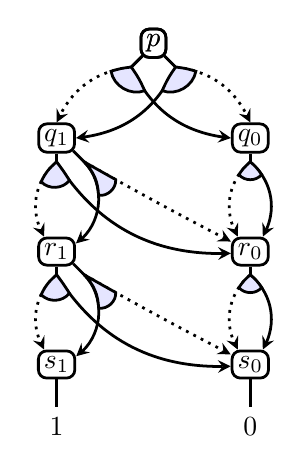
\begin{tikzpicture}[line width=1pt]
%%%%%%%%%%%%%%% p: root %%%%%%%%%%%%%%%%%%%
\node[draw,rectangle,inner sep=2pt,rounded corners=3pt] (p) {$p$};
\coordinate (pl) at ($(p.south west)+(-3pt,-3pt)$);
\coordinate (pr) at ($(p.south east)+(3pt,-3pt)$);

\draw ($(p.south west)+(1pt,1pt)$) -- (pl);
\draw ($(p.south east)+(-1pt,1pt)$) -- (pr);
%%%%%%%%%%%%%%% p: root %%%%%%%%%%%%%%%%%%%
\node[draw,rectangle,inner sep=2pt,rounded corners=3pt] (p) {$p$};
\coordinate (pl) at ($(p.south west)+(-3pt,-3pt)$);
\coordinate (pr) at ($(p.south east)+(3pt,-3pt)$);

\draw ($(p.south west)+(1pt,1pt)$) -- (pl);
\draw ($(p.south east)+(-1pt,1pt)$) -- (pr);

%%%%%%%%%%%%%%%%%%%%%%% Level 1 %%%%%%%%%%%%%%%%%%%%%%%%%%%%%%%%%%%%%%%%%%%%%%

\node[draw,rectangle,inner sep=2pt,rounded corners=3pt,anchor=north east,name=q1] 
at ($(pl)+(-20pt,-20pt)$){$q_1$};

\node[draw,rectangle,inner sep=2pt,rounded corners=3pt,anchor=north west,name=q0] 
at ($(pr)+(20pt,-20pt)$){$q_0$};


\draw[bend right=30,->,>=stealth](pl) to coordinate[pos=0.2] (pllm)(q0.west);
\draw[bend right=30,->,>=stealth,dotted](pl) to coordinate[pos=0.2] (plrm)(q1.north);

\draw[bend left=30,->,>=stealth](pr) to coordinate[pos=0.2] (prrm)(q1.east);
\draw[bend left=30,->,>=stealth,dotted](pr) to coordinate[pos=0.2] (prlm)(q0.north);


\draw[fill=blue!10] (pl) to [bend left=6]  (pllm) to [bend left=50]  (plrm) to [bend left=6] cycle;

\draw[fill=blue!10] (pr) to [bend right=6]  (prrm) to [bend right=50]  (prlm) to [bend right=6] cycle;


%%%%%%%%%%%%%%%%%%%%%%%% Level 2 %%%%%%%%%%%%%%%%%%%%%%%%%%%%%%%%%%%%%%%%

\node[draw,rectangle,inner sep=2pt,rounded corners=3pt,anchor=north,name=r1] 
at ($(q1.south)+(0pt,-30pt)$) {$r_1$};
\node[draw,rectangle,inner sep=2pt,rounded corners=3pt,anchor=north,name=r0] 
at ($(q0.south)+(0pt,-30pt)$) {$r_0$};

\coordinate (q1l) at ($(q1.south)+(0pt,-3pt)$);
\coordinate (q1r) at ($(q1.south east)+(3pt,-3pt)$);

\coordinate (q0b) at ($(q0.south)+(0pt,-3pt)$);

\draw ($(q1.south)+(0pt,0pt)$) -- (q1l);
\draw ($(q1.south east)+(-1pt,1pt)$) -- (q1r);

\draw[bend right=40,->,>=stealth,dotted](q1l) to coordinate[pos=0.3] (q1llm)(r1);
\draw[bend right=30,->,>=stealth](q1l) to coordinate[pos=0.1] (q1lrm)(r0);

\draw[fill=blue!10] (q1l) to [bend right=12]  (q1llm) to [bend right=50]  (q1lrm) to [bend right=3] cycle;

\draw[bend left=50,->,>=stealth](q1r) to coordinate[pos=0.4] (q1rlm)(r1);
\draw[bend right=1,->,>=stealth,dotted](q1r) to coordinate[pos=0.2] (q1rrm)(r0);
\draw[fill=blue!10] (q1r) to [bend left=20]  (q1rlm) to [bend right=50]  (q1rrm) to [bend left=0.2] cycle;


\draw ($(q0.south)+(0pt,0pt)$) -- (q0b);
\draw[bend right=40,->,>=stealth,dotted](q0b) to coordinate[pos=0.2] (q0blm)(r0);
\draw[bend left=40,->,>=stealth](q0b) to coordinate[pos=0.2] (q0brm)(r0);
\draw[fill=blue!10] (q0b) to [bend right=8]  (q0blm) to [bend right=50]  (q0brm) to [bend right=8] cycle;

%%%%%%%%%%%%%%%%%%%%%%%%%%%%%%%%%%%%%%%%%%%%%%%%%%%%%%%%%%%%%%%%%%%%%

%%%%%%%%%%%%%%%%%%%%%%%% Level 3 %%%%%%%%%%%%%%%%%%%%%%%%%%%%%%%%%%%%%%%%

\node[draw,rectangle,inner sep=2pt,rounded corners=3pt,anchor=north,name=s1] 
at ($(r1.south)+(0pt,-30pt)$) {$s_1$};
\node[draw,rectangle,inner sep=2pt,rounded corners=3pt,anchor=north,name=s0] 
at ($(r0.south)+(0pt,-30pt)$) {$s_0$};

\coordinate (r1l) at ($(r1.south)+(0pt,-3pt)$);
\coordinate (r1r) at ($(r1.south east)+(3pt,-3pt)$);

\coordinate (r0b) at ($(r0.south)+(0pt,-3pt)$);

\draw ($(r1.south)+(0pt,0pt)$) -- (r1l);
\draw ($(r1.south east)+(-1pt,1pt)$) -- (r1r);

\draw[bend right=40,->,>=stealth,dotted](r1l) to coordinate[pos=0.3] (r1llm)(s1);
\draw[bend right=30,->,>=stealth](r1l) to coordinate[pos=0.1] (r1lrm)(s0);

\draw[fill=blue!10] (r1l) to [bend right=12]  (r1llm) to [bend right=50]  (r1lrm) to [bend right=3] cycle;

\draw[bend left=50,->,>=stealth](r1r) to coordinate[pos=0.4] (r1rlm)(s1);
\draw[bend right=1,->,>=stealth,dotted](r1r) to coordinate[pos=0.2] (r1rrm)(s0);
\draw[fill=blue!10] (r1r) to [bend left=20]  (r1rlm) to [bend right=50]  (r1rrm) to [bend left=0.2] cycle;


\draw ($(r0.south)+(0pt,0pt)$) -- (r0b);
\draw[bend right=40,->,>=stealth,dotted](r0b) to coordinate[pos=0.2] (r0blm)(s0);
\draw[bend left=40,->,>=stealth](r0b) to coordinate[pos=0.2] (r0brm)(s0);
\draw[fill=blue!10] (r0b) to [bend right=8]  (r0blm) to [bend right=50]  (r0brm) to [bend right=8] cycle;


\node[name=1, anchor=north] at ($(s1.south)+(0pt,-10pt)$) {$1$};
\node[name=0, anchor=north] at ($(s0.south)+(0pt,-10pt)$) {$0$};
\draw[](s1) -- (1);
\draw[](s0) -- (0);
%%%%%%%%%%%%%%%%%%%%%%%%%%%%%%%%%%%%%%%%%%%%%%%%%%%%%%%%%%%%%%%%%%%%%


\end{tikzpicture}








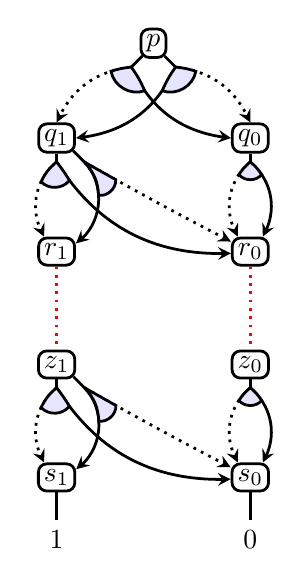
\begin{tikzpicture}[line width=1pt]
%%%%%%%%%%%%%%% p: root %%%%%%%%%%%%%%%%%%%
\node[draw,rectangle,inner sep=2pt,rounded corners=3pt] (p) {$p$};
\coordinate (pl) at ($(p.south west)+(-3pt,-3pt)$);
\coordinate (pr) at ($(p.south east)+(3pt,-3pt)$);

\draw ($(p.south west)+(1pt,1pt)$) -- (pl);
\draw ($(p.south east)+(-1pt,1pt)$) -- (pr);

%%%%%%%%%%%%%%%%%%%%%%% Level 1 %%%%%%%%%%%%%%%%%%%%%%%%%%%%%%%%%%%%%%%%%%%%%%

\node[draw,rectangle,inner sep=2pt,rounded corners=3pt,anchor=north east,name=q1] 
at ($(pl)+(-20pt,-20pt)$){$q_1$};

\node[draw,rectangle,inner sep=2pt,rounded corners=3pt,anchor=north west,name=q0] 
at ($(pr)+(20pt,-20pt)$){$q_0$};


\draw[bend right=30,->,>=stealth](pl) to coordinate[pos=0.2] (pllm)(q0.west);
\draw[bend right=30,->,>=stealth,dotted](pl) to coordinate[pos=0.2] (plrm)(q1.north);

\draw[bend left=30,->,>=stealth](pr) to coordinate[pos=0.2] (prrm)(q1.east);
\draw[bend left=30,->,>=stealth,dotted](pr) to coordinate[pos=0.2] (prlm)(q0.north);


\draw[fill=blue!10] (pl) to [bend left=6]  (pllm) to [bend left=50]  (plrm) to [bend left=6] cycle;

\draw[fill=blue!10] (pr) to [bend right=6]  (prrm) to [bend right=50]  (prlm) to [bend right=6] cycle;


%%%%%%%%%%%%%%%%%%%%%%%% Level 2 %%%%%%%%%%%%%%%%%%%%%%%%%%%%%%%%%%%%%%%%

\node[draw,rectangle,inner sep=2pt,rounded corners=3pt,anchor=north,name=r1] 
at ($(q1.south)+(0pt,-30pt)$) {$r_1$};
\node[draw,rectangle,inner sep=2pt,rounded corners=3pt,anchor=north,name=r0] 
at ($(q0.south)+(0pt,-30pt)$) {$r_0$};

\coordinate (q1l) at ($(q1.south)+(0pt,-3pt)$);
\coordinate (q1r) at ($(q1.south east)+(3pt,-3pt)$);

\coordinate (q0b) at ($(q0.south)+(0pt,-3pt)$);

\draw ($(q1.south)+(0pt,0pt)$) -- (q1l);
\draw ($(q1.south east)+(-1pt,1pt)$) -- (q1r);

\draw[bend right=40,->,>=stealth,dotted](q1l) to coordinate[pos=0.3] (q1llm)(r1);
\draw[bend right=30,->,>=stealth](q1l) to coordinate[pos=0.1] (q1lrm)(r0);

\draw[fill=blue!10] (q1l) to [bend right=12]  (q1llm) to [bend right=50]  (q1lrm) to [bend right=3] cycle;

\draw[bend left=50,->,>=stealth](q1r) to coordinate[pos=0.4] (q1rlm)(r1);
\draw[bend right=1,->,>=stealth,dotted](q1r) to coordinate[pos=0.2] (q1rrm)(r0);
\draw[fill=blue!10] (q1r) to [bend left=20]  (q1rlm) to [bend right=50]  (q1rrm) to [bend left=0.2] cycle;


\draw ($(q0.south)+(0pt,0pt)$) -- (q0b);
\draw[bend right=40,->,>=stealth,dotted](q0b) to coordinate[pos=0.2] (q0blm)(r0);
\draw[bend left=40,->,>=stealth](q0b) to coordinate[pos=0.2] (q0brm)(r0);
\draw[fill=blue!10] (q0b) to [bend right=8]  (q0blm) to [bend right=50]  (q0brm) to [bend right=8] cycle;

%%%%%%%%%%%%%%%%%%%%%%%%%%%%%%%%%%%%%%%%%%%%%%%%%%%%%%%%%%%%%%%%%%%%%

%%%%%%%%%%%%%%%%%%%%%%%% Level 2.5 %%%%%%%%%%%%%%%%%%%%%%%%%%%%%%%%%%%%%%%%
\node[draw,rectangle,inner sep=2pt,rounded corners=3pt,anchor=north,name=rr1] 
at ($(r1.south)+(0pt,-30pt)$) {$z_1$};
\node[draw,rectangle,inner sep=2pt,rounded corners=3pt,anchor=north,name=rr0] 
at ($(r0.south)+(0pt,-30pt)$) {$z_0$};

\draw[red,dotted] (r0) -- (rr0);
\draw[red,dotted] (r1) -- (rr1);
%%%%%%%%%%%%%%%%%%%%%%%% Level 3 %%%%%%%%%%%%%%%%%%%%%%%%%%%%%%%%%%%%%%%%

\node[draw,rectangle,inner sep=2pt,rounded corners=3pt,anchor=north,name=s1] 
at ($(rr1.south)+(0pt,-30pt)$) {$s_1$};
\node[draw,rectangle,inner sep=2pt,rounded corners=3pt,anchor=north,name=s0] 
at ($(rr0.south)+(0pt,-30pt)$) {$s_0$};

\coordinate (rr1l) at ($(rr1.south)+(0pt,-3pt)$);
\coordinate (rr1r) at ($(rr1.south east)+(3pt,-3pt)$);

\coordinate (rr0b) at ($(rr0.south)+(0pt,-3pt)$);

\draw ($(rr1.south)+(0pt,0pt)$) -- (rr1l);
\draw ($(rr1.south east)+(-1pt,1pt)$) -- (rr1r);

\draw[bend right=40,->,>=stealth,dotted](rr1l) to coordinate[pos=0.3] (rr1llm)(s1);
\draw[bend right=30,->,>=stealth](rr1l) to coordinate[pos=0.1] (rr1lrm)(s0);

\draw[fill=blue!10] (rr1l) to [bend right=12]  (rr1llm) to [bend right=50]  (rr1lrm) to [bend right=3] cycle;

\draw[bend left=50,->,>=stealth](rr1r) to coordinate[pos=0.4] (rr1rlm)(s1);
\draw[bend right=1,->,>=stealth,dotted](rr1r) to coordinate[pos=0.2] (rr1rrm)(s0);
\draw[fill=blue!10] (rr1r) to [bend left=20]  (rr1rlm) to [bend right=50]  (rr1rrm) to [bend left=0.2] cycle;


\draw ($(rr0.south)+(0pt,0pt)$) -- (rr0b);
\draw[bend right=40,->,>=stealth,dotted](rr0b) to coordinate[pos=0.2] (rr0blm)(s0);
\draw[bend left=40,->,>=stealth](rr0b) to coordinate[pos=0.2] (rr0brm)(s0);
\draw[fill=blue!10] (rr0b) to [bend right=8]  (rr0blm) to [bend right=50]  (rr0brm) to [bend right=8] cycle;


\node[name=1, anchor=north] at ($(s1.south)+(0pt,-10pt)$) {$1$};
\node[name=0, anchor=north] at ($(s0.south)+(0pt,-10pt)$) {$0$};
\draw[](s1) -- (1);
\draw[](s0) -- (0);
%%%%%%%%%%%%%%%%%%%%%%%%%%%%%%%%%%%%%%%%%%%%%%%%%%%%%%%%%%%%%%%%%%%%%


\end{tikzpicture}









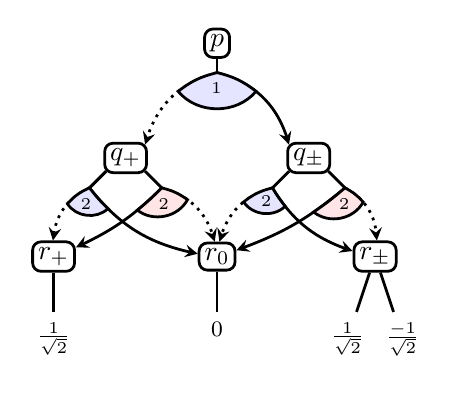
\begin{tikzpicture}[line width=1pt]
%%%%%%%%%%%%%%% p: root %%%%%%%%%%%%%%%%%%%
\node[draw,rectangle,inner sep=2pt,rounded corners=3pt] (p) {$p$};

%%%%%%%%%%%%%%%%%%%%%%% Level 1 %%%%%%%%%%%%%%%%%%%%%%%%%%%%%%%%%%%%%%%%%%%%%%

\coordinate (pB) at ($(p.south)+(0pt,-5pt)$);
\draw (p) -- (pB);

\node[draw,rectangle,inner sep=2pt,rounded corners=3pt,anchor=north east,name=q+] 
at ($(pB)+(-25pt,-25pt)$){$q_+$};
\node[draw,rectangle,inner sep=2pt,rounded corners=3pt,anchor=north west,name=q+-] 
at ($(pB)+(25pt,-25pt)$){$q_\pm$};

\coordinate  (q+NE) at ($(q+.north east)+(-1pt,-1pt)$);
\coordinate  (q+-NW) at ($(q+-.north west)+(1pt,-1pt)$);

\draw[bend right=30,->,>=stealth,dotted](pB) to coordinate[pos=0.4] 
(pBlm)(q+NE);
\draw[bend left=30, ->,>=stealth]       (pB) to coordinate[pos=0.4] 
(pBrm)(q+-NW);

\draw[fill=blue!10] (pB) to [bend right=12]  (pBlm) to [bend right=50]  (pBrm) to [bend right=12] cycle;

\node[anchor=north,font=\footnotesize] at (pB) {$\xvar_1$};





\coordinate  (q+SW) at ($(q+.south west)+(1pt,1pt)$);
\coordinate (q+L) at ($(q+.south west)+(-5pt,-5pt)$);
\draw (q+SW) -- (q+L);

\coordinate  (q+SE) at ($(q+.south east)+(-1pt,1pt)$);
\coordinate (q+R) at ($(q+.south east)+(5pt,-5pt)$);

\coordinate  (q+-SW) at ($(q+-.south west)+(1pt,1pt)$);
\coordinate (q+-L) at ($(q+-.south west)+(-5pt,-5pt)$);

\coordinate  (q+-SE) at ($(q+-.south east)+(-1pt,1pt)$);
\coordinate (q+-R) at ($(q+-.south east)+(5pt,-5pt)$);



\draw (q+SW) -- (q+L);
\draw (q+SE) -- (q+R);

\draw (q+-SW) -- (q+-L);
\draw (q+-SE) -- (q+-R);

%%%%%%%%%%%%%%%%%%%%%%% Level 2 %%%%%%%%%%%%%%%%%%%%%%%%%%%%%%%%%%%%%%%%%%%%%%


\node[draw,rectangle,inner sep=2pt,rounded corners=3pt,anchor=north east,name=r+] 
at ($(q+SE)+(-25pt,-25pt)$){$r_+$};

\node[draw,rectangle,inner sep=2pt,rounded corners=3pt,anchor=north east,name=r+-] 
at ($(q+-SE)+(25pt,-25pt)$){$r_\pm$};

\node[draw,rectangle,inner sep=2pt,rounded corners=3pt,name=r0] 
at (r+-| p){$r_0$};

\draw[bend right=30,->,>=stealth,dotted](q+L) to coordinate[pos=0.4] 
(q+Llm)(r+);
\draw[bend right=20,->,>=stealth](q+L) to coordinate[pos=0.2] 
(q+Lrm)(r0);
\draw[fill=blue!10] (q+L) to [bend right=12]  (q+Llm) to [bend right=50]  (q+Lrm) to [bend left=4] cycle;
\node[anchor=north,font=\footnotesize] at ($(q+L)+(-1pt,0pt)$) {$\xvar_2$};


\draw[bend left=10,->,>=stealth](q+R) to coordinate[pos=0.3] 
(q+Rlm)(r+);
\draw[bend left=30,->,>=stealth,dotted](q+R) to coordinate[pos=0.35] 
(q+Rrm)(r0);
\draw[fill=red!10] (q+R) to [bend left=3]  (q+Rlm) to [bend right=50]  (q+Rrm) to [bend right=10.5] cycle;
\node[anchor=north,font=\footnotesize] at ($(q+R)+(1pt,0pt)$) {$\xvar_2$};


\draw[bend right=30,->,>=stealth,dotted](q+-L) to coordinate[pos=0.4] 
(q+-Llm)(r0);
\draw[bend right=20,->,>=stealth](q+-L) to coordinate[pos=0.2] 
(q+-Lrm)(r+-);
\draw[fill=blue!10] (q+-L) to [bend right=12]  (q+-Llm) to [bend right=50]  (q+-Lrm) to [bend left=4] cycle;
\node[anchor=north,font=\footnotesize] at ($(q+-L)+(-2pt,1pt)$) {$\xvar_2$};


\draw[bend left=10,->,>=stealth](q+-R) to coordinate[pos=0.3] 
(q+-Rlm)(r0);
\draw[bend left=30,->,>=stealth,dotted](q+-R) to coordinate[pos=0.35] 
(q+-Rrm)(r+-);
\draw[fill=red!10] (q+-R) to [bend left=3]  (q+-Rlm) to [bend right=50]  (q+-Rrm) to [bend right=10.5] cycle;
\node[anchor=north,font=\footnotesize] at ($(q+-R)+(0pt,0pt)$) {$\xvar_2$};



%%%%%%%%%%%%%%%% Leafs %%%%%%%%%%%%%%%%


\node[anchor=north,font=\footnotesize,name=leafr+] at ($(r+)+(0pt,-20pt)$) {$\frac1{\sqrt2}$};
\draw (r+) -- (leafr+);

\node[anchor=north,font=\footnotesize,name=leafr0] at ($(r0)+(0pt,-20pt)$) {$0$};
\draw (r0) -- (leafr0);

\node[anchor=north,font=\footnotesize,name=leftleafr+-] at ($(r+-)+(-10pt,-20pt)$) {$\frac1{\sqrt2}$};
\draw (r+-) -- (leftleafr+-);

\node[anchor=north,font=\footnotesize,name=rightleafr+-] at ($(r+-)+(+10pt,-20pt)$) {$\frac{-1}{\sqrt2}$};
\draw (r+-) -- (rightleafr+-);

\end{tikzpicture}



\input tmp
\end{document}

